\section{java.util.Map}

\frame{\frametitle{java.util.Map}
\begin{center}
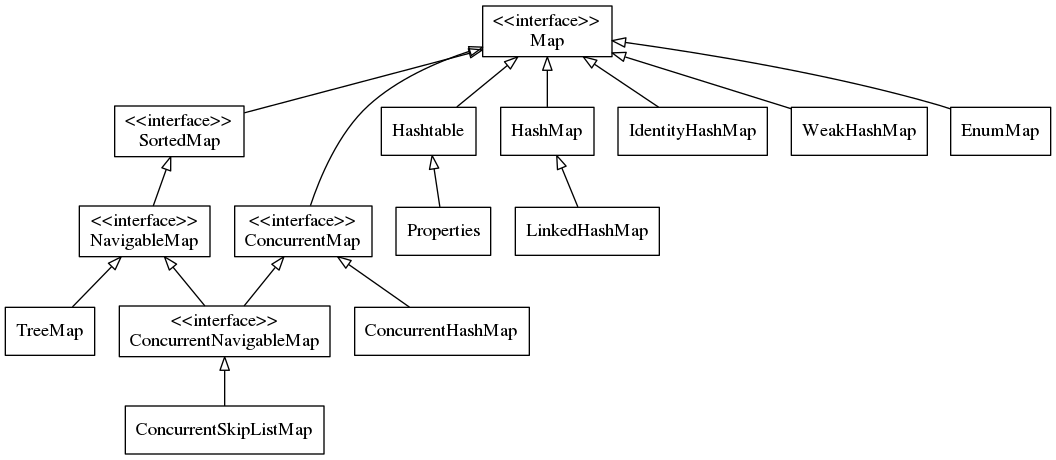
\includegraphics[width=0.9\textwidth]{java.util.Map/java_util_Map_overview}
\end{center}
}

\frame{
\frametitle{HashMap}
\begin{center}
  \begin{itemize}[<+->]
    \item seit 1.2
    \item null keys und values erlaubt
    \item wie Hashtable, aber mit nulls und nicht thread-safe
    \item get/put in \O{1}
    \item nicht thread-safe
    \item fail-fast iterator
  \end{itemize}
\end{center}
}

\begin{frame}[fragile]
\frametitle{HashMap - interne Struktur}
\begin{itemize}[<+->]
  \item capacity = Anzahl an buckets, initialCapacity = Start capacity
  \item loadFactor = Ab wann automatisch rehash
  \item rehash: interne Datenstruktur wird neu gebaut $\Rightarrow$ Kapazität steigt um Faktor 2
  \item Konstruktor: initialCapacity und loadFactor \\
	$DEFAULT_LOAD_FACTOR = 0.75f$ \\
	$DEFAULT_INITIAL_CAPACITY = 1 << 4; // = 16$
  \item wenn $number\ entries \geq loadFactor * capacity$ dann rehash
  \item wenn viele puts, dann sollte initialCapacity groß genug sein, um Anzahl an rehashes klein zu halten
  \item aber initialCapacity nicht zu hoch und loadFactor nicht zu niedrig setzen, sonst zu viele rehashes
\end{itemize}
\end{frame}

\frame{
\frametitle{HashMap - Zugriffszeiten}
\begin{center}
  \begin{tabular}{l|l}
  Operation        & Laufzeit \\\hline
  get              & \O{1} \\
  put              & \O{1} \\
  \end{tabular}
\end{center}
}

\frame{
\frametitle{HashMap - Wann nehmen?}
\begin{center}
  Synchronisation egal, \\\pause
  Ordnung egal, \\\pause
  oft get/put
\end{center}
}

\frame{
\frametitle{Map - Übersicht}
\begin{center}
  \begin{tabular}{l|c|c|c|c}
                       & thread-safe &  Iterator & Reihenfolge & null value \\\hline
  HashMap              &     nein    & fail-fast &             &   erlaubt  \\
  \end{tabular}
\end{center}
}
